\documentclass[../main.tex]{subfiles}

% ======================== Document: Empirical Strategy ======================== %

\begin{document}
\section{Empirical Strategy}
\label{sec:empirical_strategy}

\subsection{Data}

I employ a novel administrative dataset from the Canadian Intellectual Property Office, the IP Horizons Patent Researcher Datasets\nocite{canadianintellectualpropertyoffice23}. The data identify patents in Canada from 1860 to 2023, with information on when the application for the patent was filed and granted as well as the parties involved in the application. Parties can be identified to provinces based on their location, which can be in Canada or other countries. 

% As mentioned on \Section, parties involved in a patent application can be agents, inventors, owners or applicants.

With these data, I compute quarterly patent application counts at the province level from January 2001 to June 2021, based on the application filing date. This period corresponds to the modern Canadian intellectual property institutional context, as reviewed on Section \ref{sec:institutional_background}. Further, limiting to a period smaller than twenty years reduces the possibility of double counting patent renewal applications. I assign patents to provinces based on where the majority of parties involved in a patent application report their location\footnote{Patent applications without information of party provinces or with an equal number of interested parties from two provinces are dropped from the sample.}. I only include the first two quarters of 2021 the last two quarters present an unusual downward trend for all provinces in late 2021, suggesting patent applications are yet to be updated. Further, I drop Newfoundland and Labrador, Prince Edward Island, Yukon and Nunavut due to missing observations on most explanatory variables. 

% Note: state the percentages of patents with missing data on parties and dropped patents due to ties. 

The explained variable of interest is the count of patent applications. Further, to allow for heterogeneity in treatment, I separate patents by their International Patent Classification (IPC) section. I then consider the count of patent applications for each IPC section as separate explained variables for some models.

For my explanatory variables, I extract province-level data at the monthly frequency from Statistics Canada and later aggregate quarterly. These include data from the Labour Force Survey (LFS), such as labour force characteristics, employment wages, among others\nocite{lfs_lfc_table,lfs_employee_wages,statisticscanada24,statisticscanada24b}. Further, I also consider the consumer price index\nocite{cpi}, international merchandise exports and imports\nocite{statisticscanada24g}, retail, wholesale and manufacturing trade sales\nocite{retail_trade_sales,wholesale_trade,manufacturing_sales}, food services receipts\nocite{statisticscanada24c}, the new housing price index\nocite{statisticscanada24a} and electric power generation\nocite{statisticscanada24f,statisticscanada08}. I also include the number of business insolvencies as reported by \textcite{insolvency24} (\citeyear{insolvency24}) and the number of foreign parties involved in patent applications, which I obtain from the IP Horizons data. I aggregate data at the quarterly level by summing all variables except the consumer and new housing indices, for which I take arithmetic averages. Table \ref{tab:descriptive_statistics} presents descriptive statistics for patents and all explanatory variables.

\begin{table}[h]
    \centering
    \begin{threeparttable}
        \caption{Descriptive statistics for the province-quarter sample}
        \label{tab:descriptive_statistics}
        
\begin{tabular}[t]{lrrrrr}
\toprule
  & Mean & SD & Min & Median & Max\\
\midrule
Ln +1 Patent applications & \num{4.261} & \num{1.405} & \num{1.099} & \num{4.107} & \num{6.691}\\
Ln Full-time employment & \num{8.026} & \num{1.034} & \num{6.726} & \num{7.831} & \num{9.814}\\
Ln Median wage & \num{2.949} & \num{0.192} & \num{2.523} & \num{2.956} & \num{3.395}\\
CPI & \num{119.145} & \num{12.668} & \num{95.400} & \num{119.400} & \num{148.900}\\
Ln +1 Business insolvencies & \num{4.403} & \num{1.396} & \num{0.693} & \num{4.197} & \num{6.957}\\
Ln Intl. exports & \num{15.810} & \num{1.139} & \num{13.694} & \num{15.848} & \num{17.804}\\
Ln Intl. imports & \num{15.646} & \num{1.198} & \num{13.715} & \num{15.369} & \num{18.372}\\
Ln Retail sales & \num{15.963} & \num{1.028} & \num{14.424} & \num{15.774} & \num{17.913}\\
Ln Wholesale sales & \num{15.910} & \num{1.292} & \num{13.907} & \num{15.892} & \num{18.490}\\
Ln Manufacturing sales & \num{16.027} & \num{1.179} & \num{14.398} & \num{15.729} & \num{18.213}\\
Ln International travellers & \num{12.470} & \num{1.779} & \num{4.344} & \num{12.387} & \num{15.929}\\
Ln Arriving vehicles & \num{11.944} & \num{3.562} & \num{0.000} & \num{12.516} & \num{15.801}\\
Ln Electric power generation & \num{16.213} & \num{0.997} & \num{14.344} & \num{16.219} & \num{17.990}\\
Ln Average actual hours & \num{3.545} & \num{0.050} & \num{3.311} & \num{3.550} & \num{3.676}\\
New housing price index & \num{88.064} & \num{16.987} & \num{42.900} & \num{94.250} & \num{129.500}\\
Ln Food services receipts & \num{13.737} & \num{1.108} & \num{12.255} & \num{13.575} & \num{15.857}\\
Ln Average job tenure & \num{4.636} & \num{0.088} & \num{4.399} & \num{4.653} & \num{4.830}\\
Ln +1 Foreign patent parties & \num{3.609} & \num{1.918} & \num{0.000} & \num{3.842} & \num{6.671}\\
\bottomrule
\end{tabular}
}
        \begin{tablenotes}
            \small
            \item \textit{Notes}: All statistics based on a balanced panel of $N$ = 656 province-quarter observations from 2001Q1 to 2021Q2. The sample includes all Canadian provinces except Newfoundland and Labrador, Prince Edward Island, Yukon and Nunavut.
        \end{tablenotes}
    \end{threeparttable}
  \end{table}
  

\subsection{Empirical Strategy}

The AITC, as an investor tax credit, did not directly affect innovation inputs such as R\&D expenditures. However, since it directly provided cheaper financing for innovative firms, it may have affected innovation output in the form of patent applications. To estimate the effect of the AITC on patent applications, I implement a two-way fixed effects (TWFE) difference-in-differences (DD) design, where I define treatment and control groups based on the period the program was passed, which was 2017Q1 (January 2017) \parencite{albertaeconomicdevelopmentandtrade17}. While the first investment elegibility date was in 2016Q2 (April 2016)

The treatment group is Alberta, and the treatment period is composed of all periods after 2017Q1. The control group is all remaining Canadian provinces in the sample. Treated observations are those from Alberta after 2017Q1, where I believe the AITC affected Albertan patent applications. The DD design is implemented in a regression framework, according to the general specification below.

\begin{equation}
    \label{eq:dd_model}
    \ln(P_{it} + 1) = \theta_i + \theta_t + \beta \ T_{it} + \mathbb{x}_{it}^{'} \gamma + u_{it}
\end{equation}

where $P_{it}$ is the explained variable; in most specifications, $P_{it}$ is the number of patents filed in a province $i$ and period $t$. $\theta_i$ and $\tau_t$ are sets of province and period fixed effects. I use a natural logarithm transformation along with the addition of one to correct for provinces with small amounts of patent applications on some periods. $T_{it}$ is a binary variable equal to unity for observations for treated observations and zero otherwise. Hence, the estimated parameter $\hat{\beta}$ is the coefficient of interest, which is my estimate for the average treatment effect of the AITC on the explained variable. $\mathbf{x}_{it}$ is a vector of time and province-varying controls, as described in the previous subsection, and $\gamma$ is the associated vector of parameters. $u_{it}$ is a stochastic error term which varies between provinces and periods. For my results, I cluster standard errors at the province and period level. 

\begin{table}[htbp!]
    \centering
    \begin{threeparttable}
        \caption{Differences in means between treated and control provinces in province-quarter panel}
        \label{tab:diff_means_quarterly}
        
\begin{tabular}[t]{llrr}
\toprule
Treatment &   & Pre & Post\\
\midrule
Control & Ln +1 Patent applications & \num{4.122} & \num{4.059}\\
 & Ln +1 Interested parties & \num{5.683} & \num{5.464}\\
 & Ln +1 Inventors & \num{301.511} & \num{292.143}\\
 & Ln +1 Applicants & \num{158.663} & \num{139.122}\\
 & Ln +1 Owners & \num{330.344} & \num{150.204}\\
 & Ln +1 Total population & \num{8.632} & \num{8.731}\\
 & Ln +1 Foreign patent parties & \num{3.405} & \num{3.189}\\
 & Ln +1 Section A applications & \num{2.550} & \num{2.596}\\
 & Ln +1 Section B applications & \num{2.238} & \num{2.037}\\
 & Ln +1 Section C applications & \num{1.464} & \num{1.306}\\
 & Ln +1 Section D applications & \num{0.349} & \num{0.185}\\
 & Ln +1 Section E applications & \num{1.496} & \num{1.512}\\
 & Ln +1 Section F applications & \num{1.618} & \num{1.417}\\
 & Ln +1 Section G applications & \num{1.840} & \num{1.993}\\
 & Ln +1 Section H applications & \num{1.620} & \num{1.380}\\
 & Ln +1 Multiple section applications & \num{2.879} & \num{2.972}\\
Treatment & Ln +1 Patent applications & \num{5.379} & \num{5.254}\\
 & Ln +1 Interested parties & \num{6.800} & \num{6.665}\\
 & Ln +1 Inventors & \num{314.787} & \num{383.571}\\
 & Ln +1 Applicants & \num{219.607} & \num{194.810}\\
 & Ln +1 Owners & \num{378.721} & \num{211.762}\\
 & Ln +1 Total population & \num{9.043} & \num{9.236}\\
 & Ln +1 Foreign patent parties & \num{5.650} & \num{4.750}\\
 & Ln +1 Section A applications & \num{2.704} & \num{2.896}\\
 & Ln +1 Section B applications & \num{2.927} & \num{3.020}\\
 & Ln +1 Section C applications & \num{2.632} & \num{2.633}\\
 & Ln +1 Section D applications & \num{0.190} & \num{0.258}\\
 & Ln +1 Section E applications & \num{4.073} & \num{3.761}\\
 & Ln +1 Section F applications & \num{2.510} & \num{2.406}\\
 & Ln +1 Section G applications & \num{3.075} & \num{2.853}\\
 & Ln +1 Section H applications & \num{1.950} & \num{1.789}\\
 & Ln +1 Multiple section applications & \num{4.100} & \num{4.111}\\
\bottomrule
\end{tabular}
}
        \begin{tablenotes}
            \small
            \item \textit{Notes}: Calculations based on a balanced panel of $N$ = 656 province-monthly observations from 2001Q1 to 2021Q2. The sample includes all Canadian provinces except Newfoundland and Labrador, Prince Edward Island, Yukon and Nunavut. The treatment group is Alberta, and the control group is made from all remaining provinces. Post-intervention periods are those after April 2016 (2016Q2).
        \end{tablenotes}
    \end{threeparttable}

\end{table}

Tables \ref{tab:diff_means_quarterly} presents the difference in means between treated and control provinces for the province-quarter panel for all considered explained variables. This presents the simplest version of the DD model, where I compare the average number of patent applications between Alberta and the control provinces before and after the AITC intervention. This simple comparison suggests a small or null effect; the regression analysis described above will provide a more robust DD estimate. 

The key identifying assumption of the DD design is that, absent the AITC intervention, the trend of patents in Alberta would follow a similar pattern to control provinces. Figure \ref{fig:quarterly_common_trends} shows the quarterly time series of patent applications between Alberta and control provinces from 2001Q1 to 2021Q2. This visual representation of the trends shows that Alberta's patent applications follow a similar pattern to control provinces before the intervention, however, some deviations are present before 2016Q2.

\begin{figure}[h]
    \centering
    \caption{Quarterly time series of patent applications between treatment and control groups}
    \label{fig:quarterly_common_trends}
    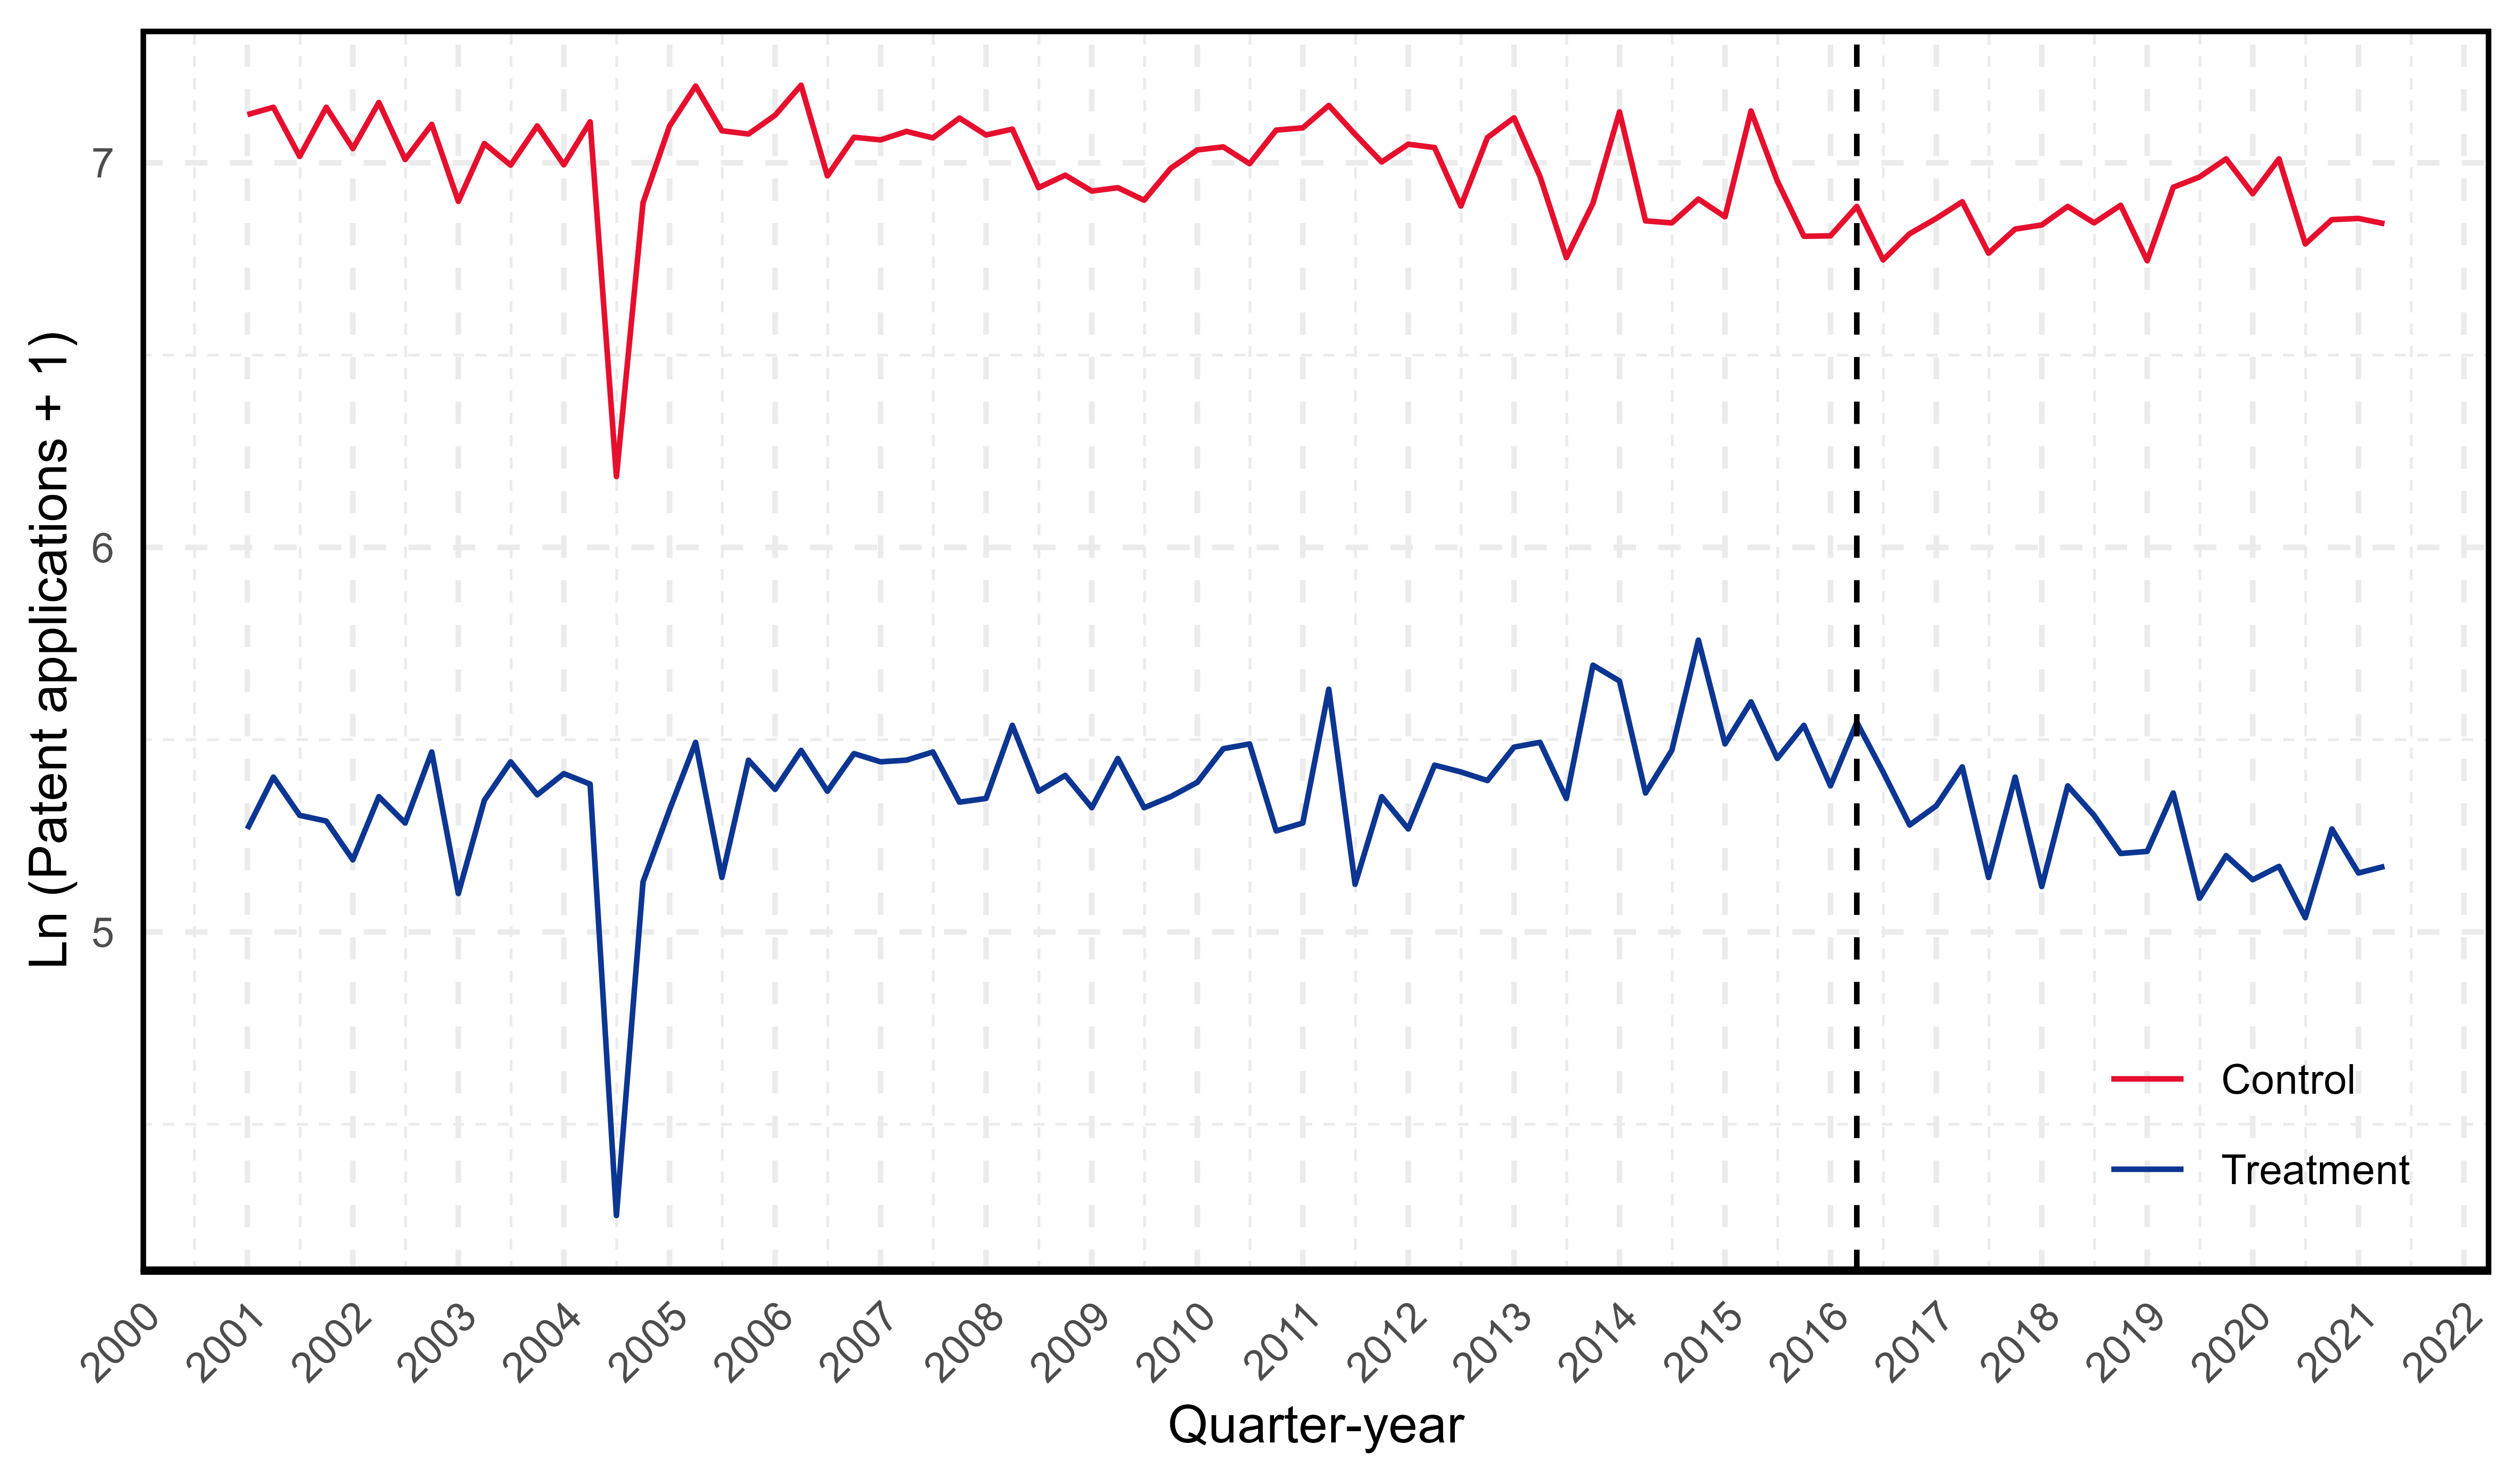
\includegraphics{\subfix{../../figures/quarterly_common_trends.png}}
    \begin{minipage}{0.9\textwidth}
        \footnotesize
        \textit{Notes}: The figure shows the quarterly time series of patent applications between the treatment and control groups from 2001Q1 to 2021Q2. The vertical line represents the start of the AITC intervention (first expense eligibility date) in April 2016. The treatment group is Alberta, and the control group is made from all remaining provinces except NL, PE, YT and NU. 
    \end{minipage}
\end{figure}

To allay the concern of unobservable factors impacting patent application trends across provinces, I estimate event study regressions following Equation \ref{eq:event_study} below and provide supporting evidence for causal identification of $\hat{\beta}$.

\begin{equation}
    \label{eq:event_study}
   \ln(P_{it} + 1) = \theta_i + \tau_t + \mathbb{\beta_t}(t \cdot A_t) + \mathbb{x}_{it}^{'}\gamma + u_{it}
\end{equation}

$\theta_i, \tau_t, \mathbf{x}_{it}, \gamma$ and $u_{it}$ represent the same as in Equation \ref{eq:dd_model}. $t$ is a set of binary variables for each of the periods for which there is data available, with the reference level set to one period before AITC eligibility (March 2016). $A_t$ is a binary variable equal to unity if the observation is mapped to Alberta and zero otherwise. $t\cdot A_t$ is the interaction term between these two variables, and $\beta_t$ is the associated vector of coefficients, which will show the difference between the treatment and control groups in the explained variable for all $t$. For these regressions, I show the values of the interaction terms in event study plots, along with their 95\% confidence intervals. I cluster standard errors at the province and period level.

Evidence in favour of the identifying assumption will be observed if the interaction terms before April 2016 are not statistically significant. This supports the idea that Alberta had no significant differences in the trend of patent applications to other provinces before the intervention. Thus, I use the event study regressions to provide evidence of the causal identification of the average treatment effect of the AITC on patent applications. In section \ref{sec:results}, I justify the causal identification of the AITC effect by showing that the interaction terms before the intervention are not statistically significant. Further, I use event study regressions in the form of \ref{eq:event_study} examine the effectiveness of the AITC by looking at post-treatment interaction terms, which should show statistically significant differences if the AITC affected Albertan patent applications.

\subsection{Patent parties and province-month panel}

I perform two main robustness checks on DD and event study analyses to ensure the validity of my results. First, to the extent that results may be driven by the arbitrary mapping of patents to provinces, I consider the number of Canadian parties involved in a patent application as an alternative explained variable. I separate parties by type (all parties, inventors, owners and applicants\footnote{I do not consider agents as a separate category due to them typically being hired legal professionals, which may not be informative about the innovative capacity of who files for the patent.}.) to understand the effect of the AITC on the innovative capacity of different groups. Table \ref{tab:diff_means_quarterly} also presents the difference in means between treated and control provinces for the province-quarter panel for parties involved in patent applications.

Second, I reestimate models on a province-month panel, to ensure that the results are not driven by the aggregation of data at the quarterly level. This panel allows for a more granular analysis of the effects of the AITC on patent applications, however, it is susceptible to noise due to the smaller number of observations, especially for the event study regressions. I present descriptive statistics of the monthly data in \ref{sec:appendixa}. 
\end{document}